\section{Anhang}
\label{sec:Anhang}
\subsection{Originaldaten}

\begin{figure}[H]
  \centering
  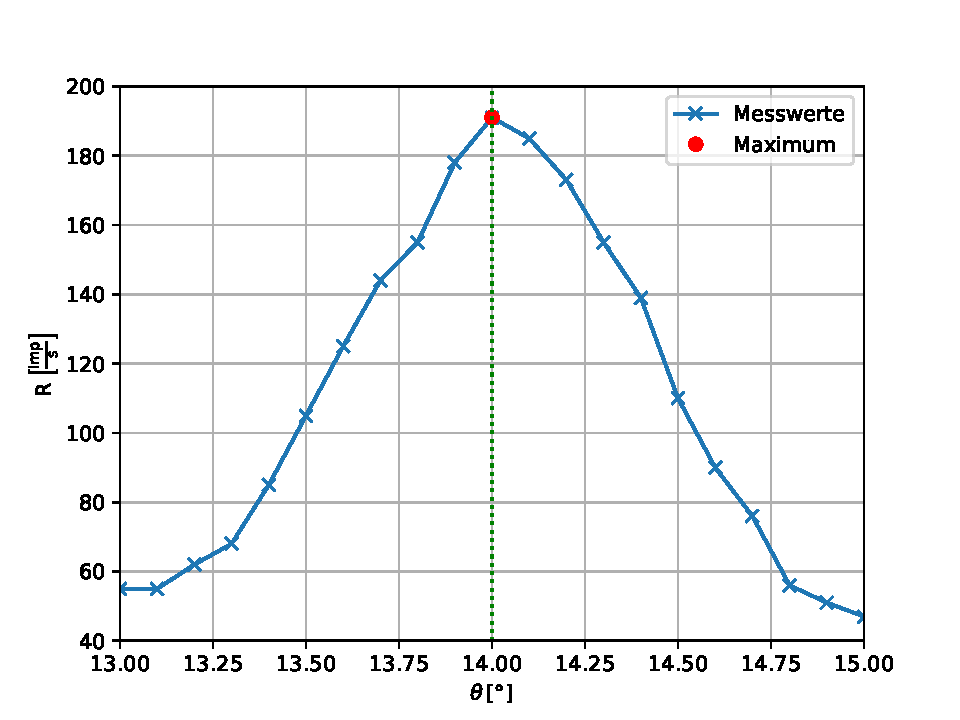
\includegraphics[width=\textwidth, angle=270, origin=c]{"content/Bilder/Bragg.jpg"}
  \caption{Messdaten für die Bragg-Bedingung.}
  \label{fig:Messungen_1}
\end{figure}
\begin{figure}[H]
    \centering
    \includegraphics[width=\textwidth, angle=270, origin=c]{"content/Bilder/Emission1.jpg"}
    \caption{Messdaten für das Emissionsspektrum Seite 1.}
    \label{fig:Messungen_2}
  \end{figure}
  \begin{figure}[H]
    \centering
    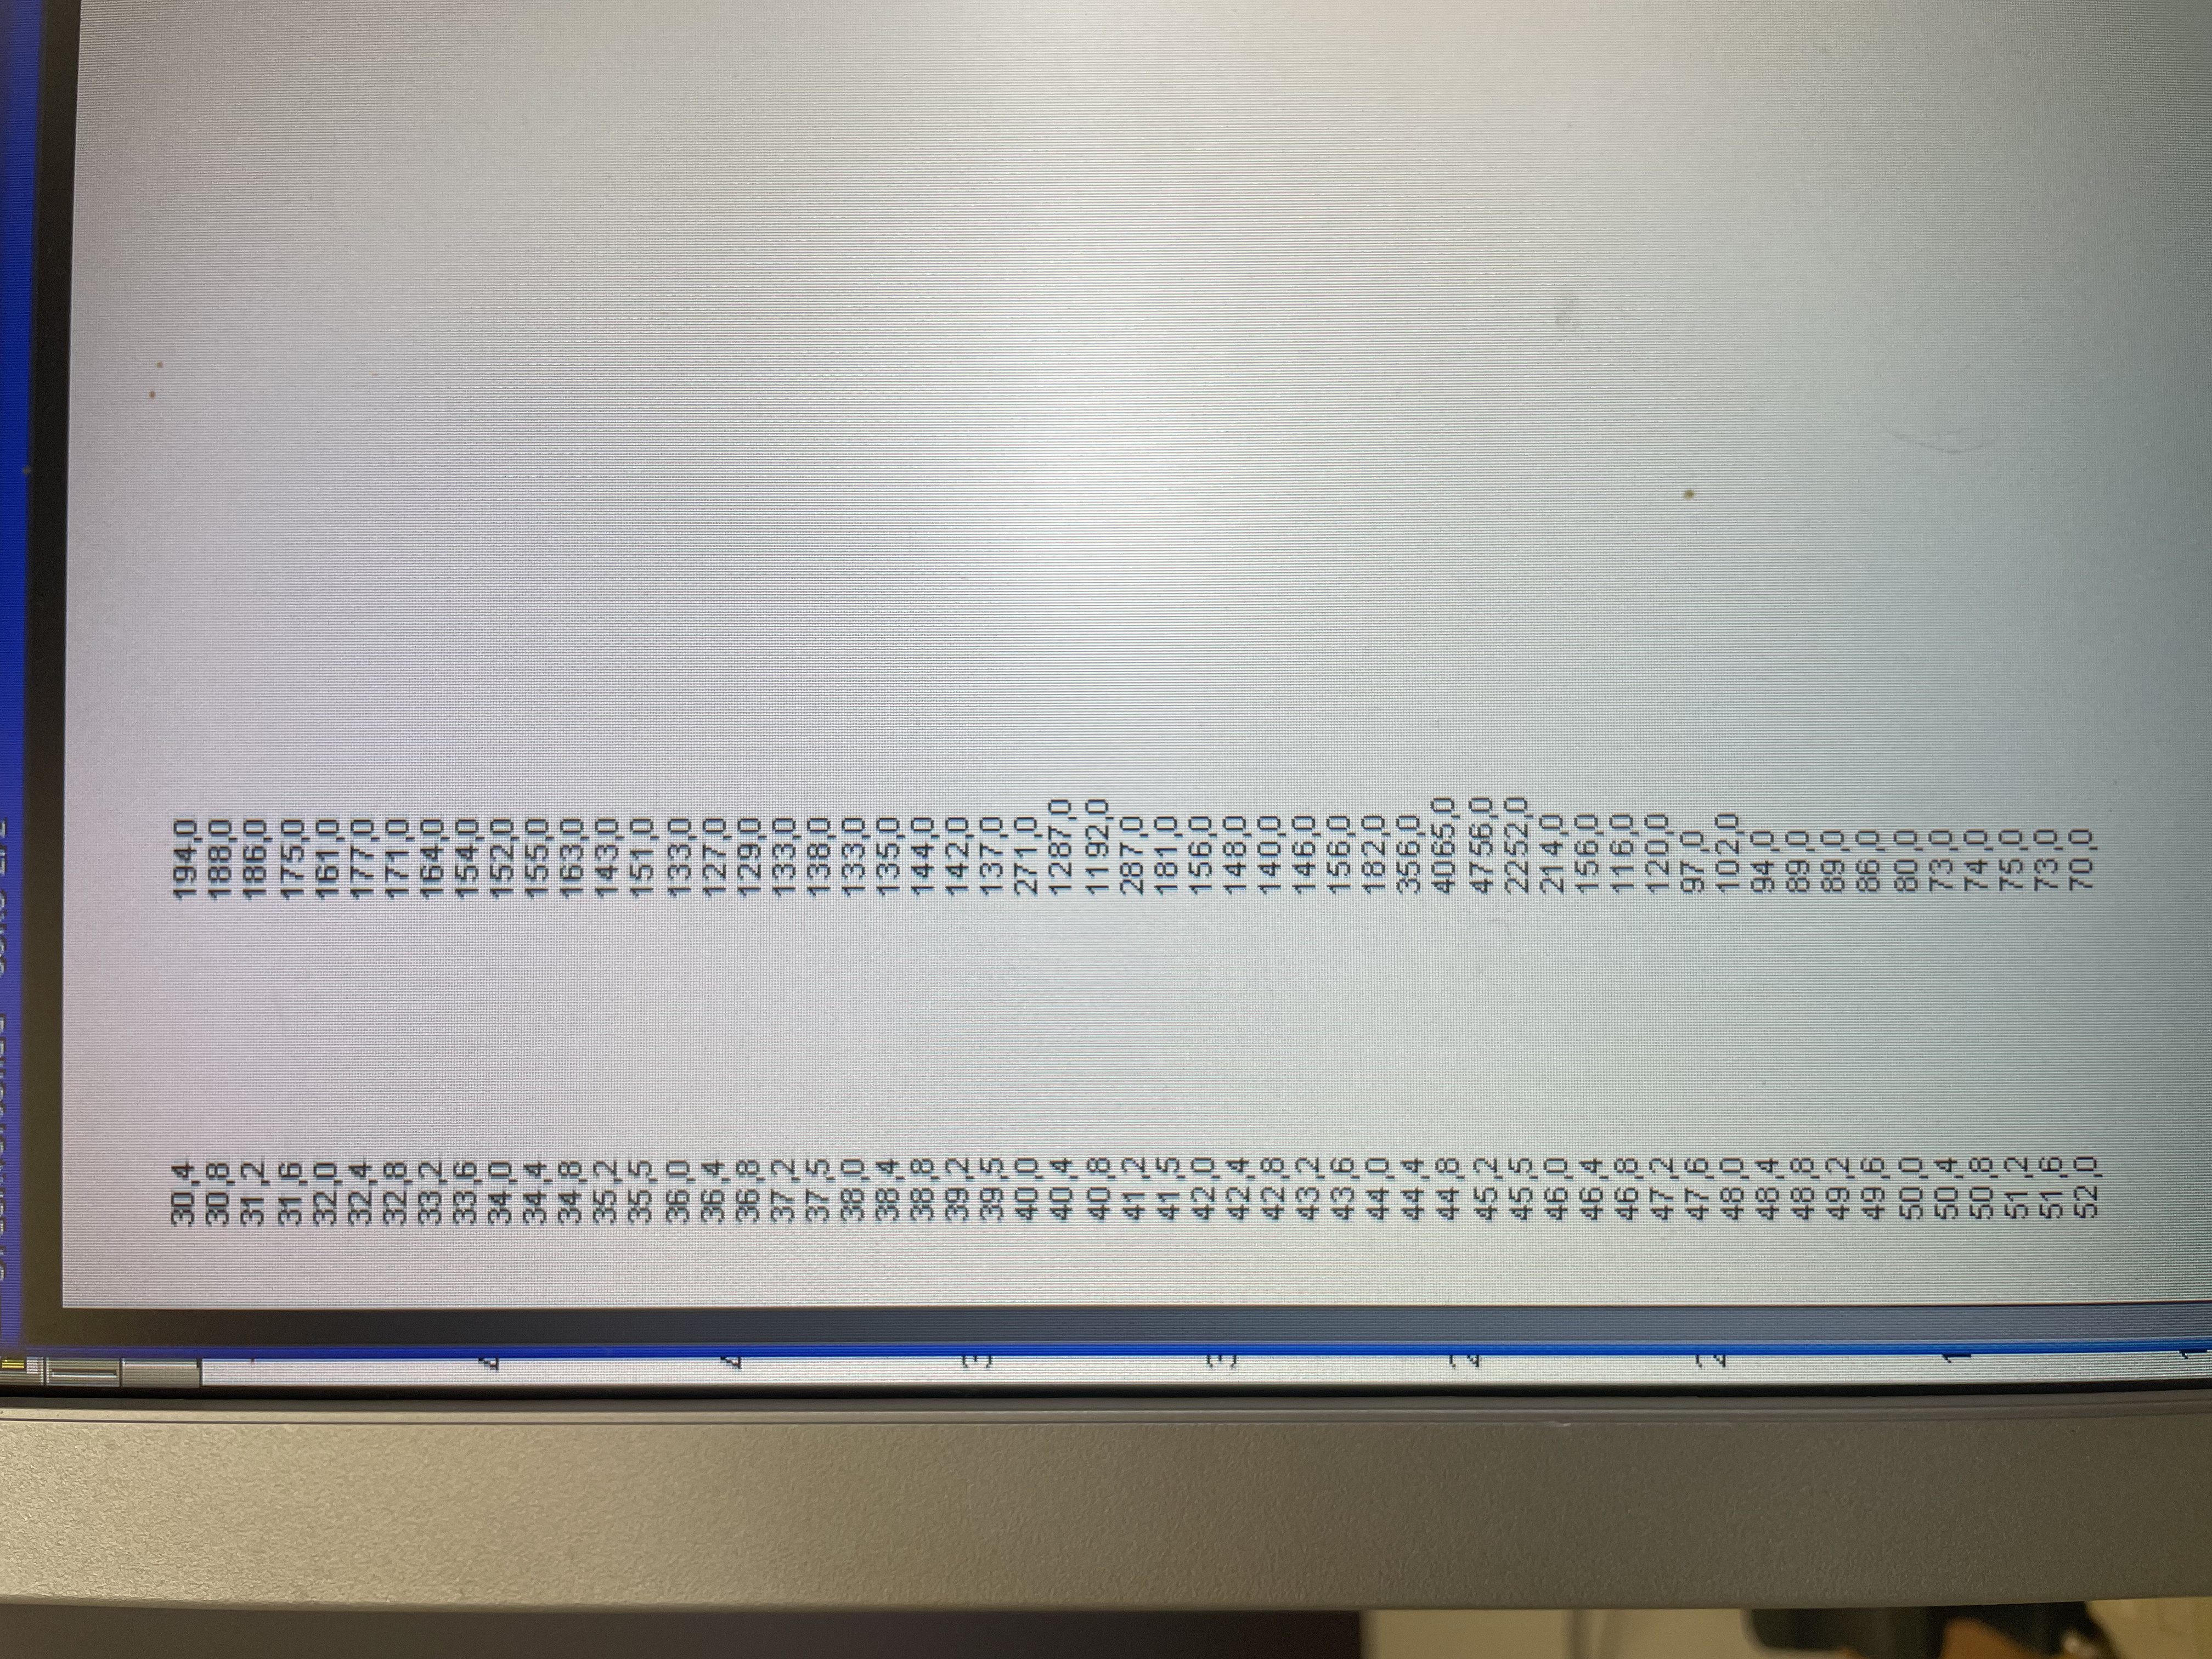
\includegraphics[width=\textwidth, angle=270, origin=c]{"content/Bilder/Emission2.jpg"}
    \caption{Messdaten für das Emissionsspektrum Seite 2.}
    \label{fig:Messungen_3}
  \end{figure}
  \begin{figure}[H]
    \centering
    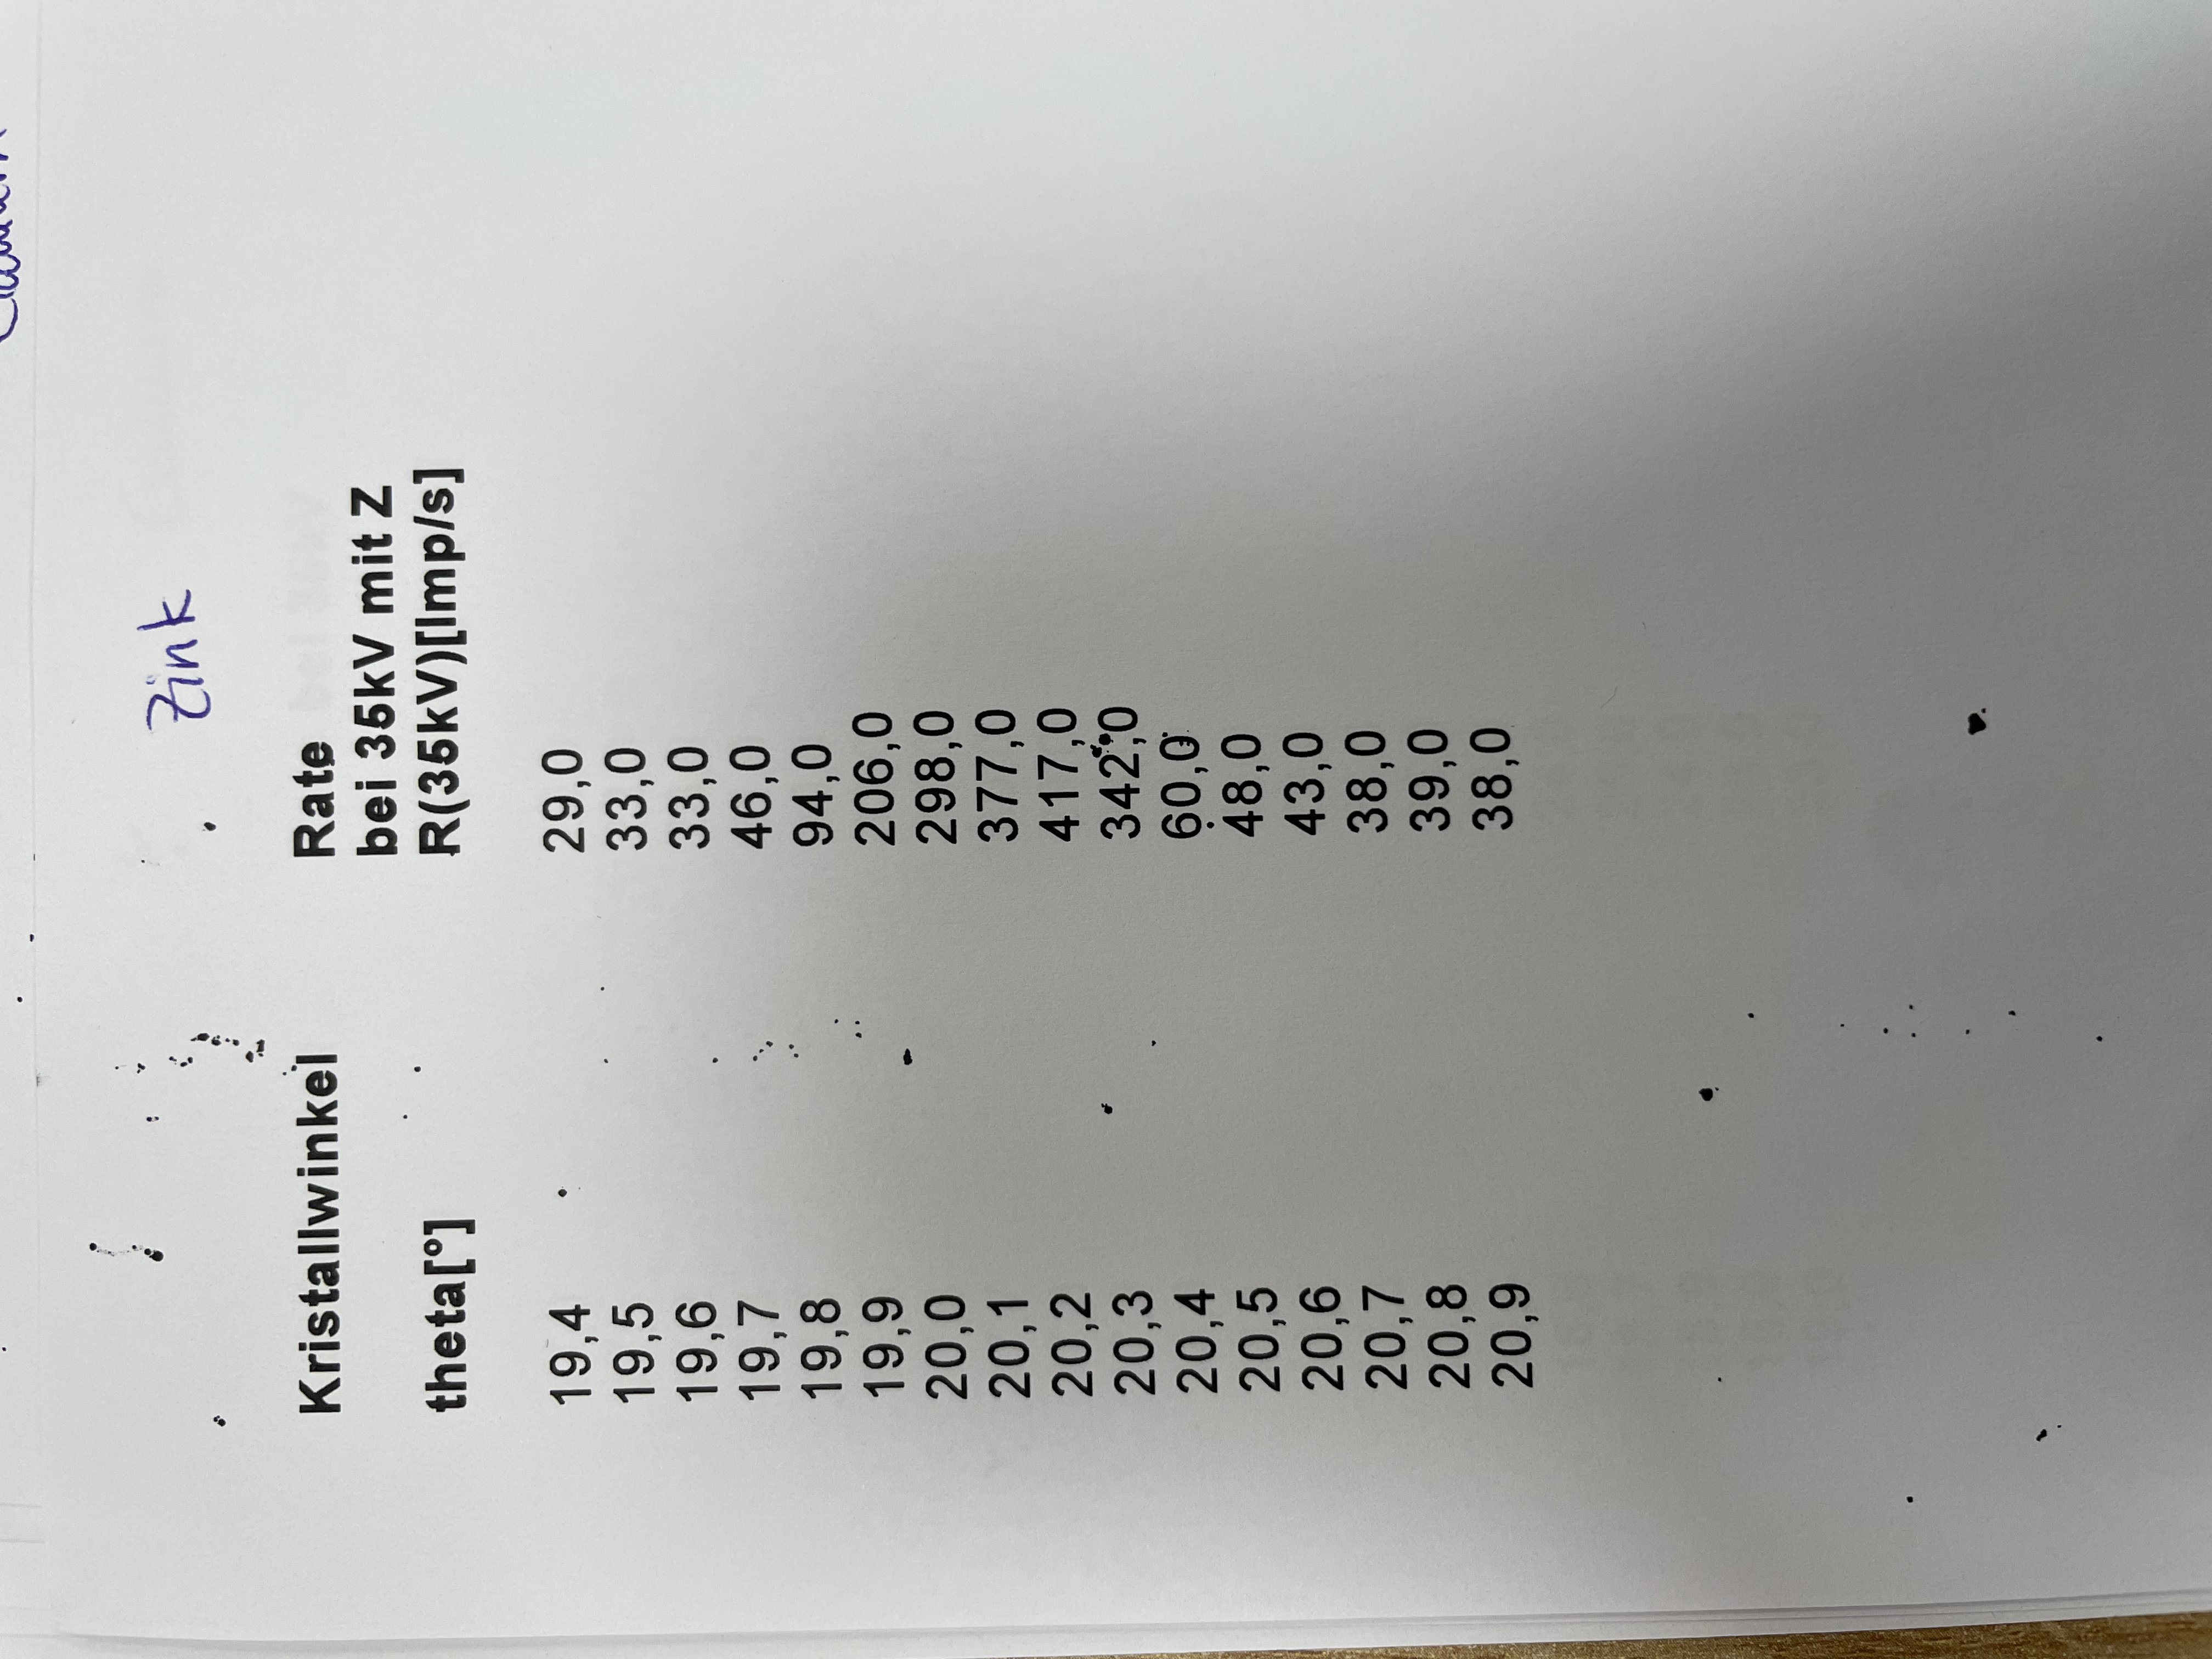
\includegraphics[width=\textwidth, angle=270, origin=c]{"content/Bilder/Zink.jpg"}
    \caption{Messdaten für den Zink-Absorber.}
    \label{fig:Messungen_4}
  \end{figure}
  \begin{figure}[H]
    \centering
    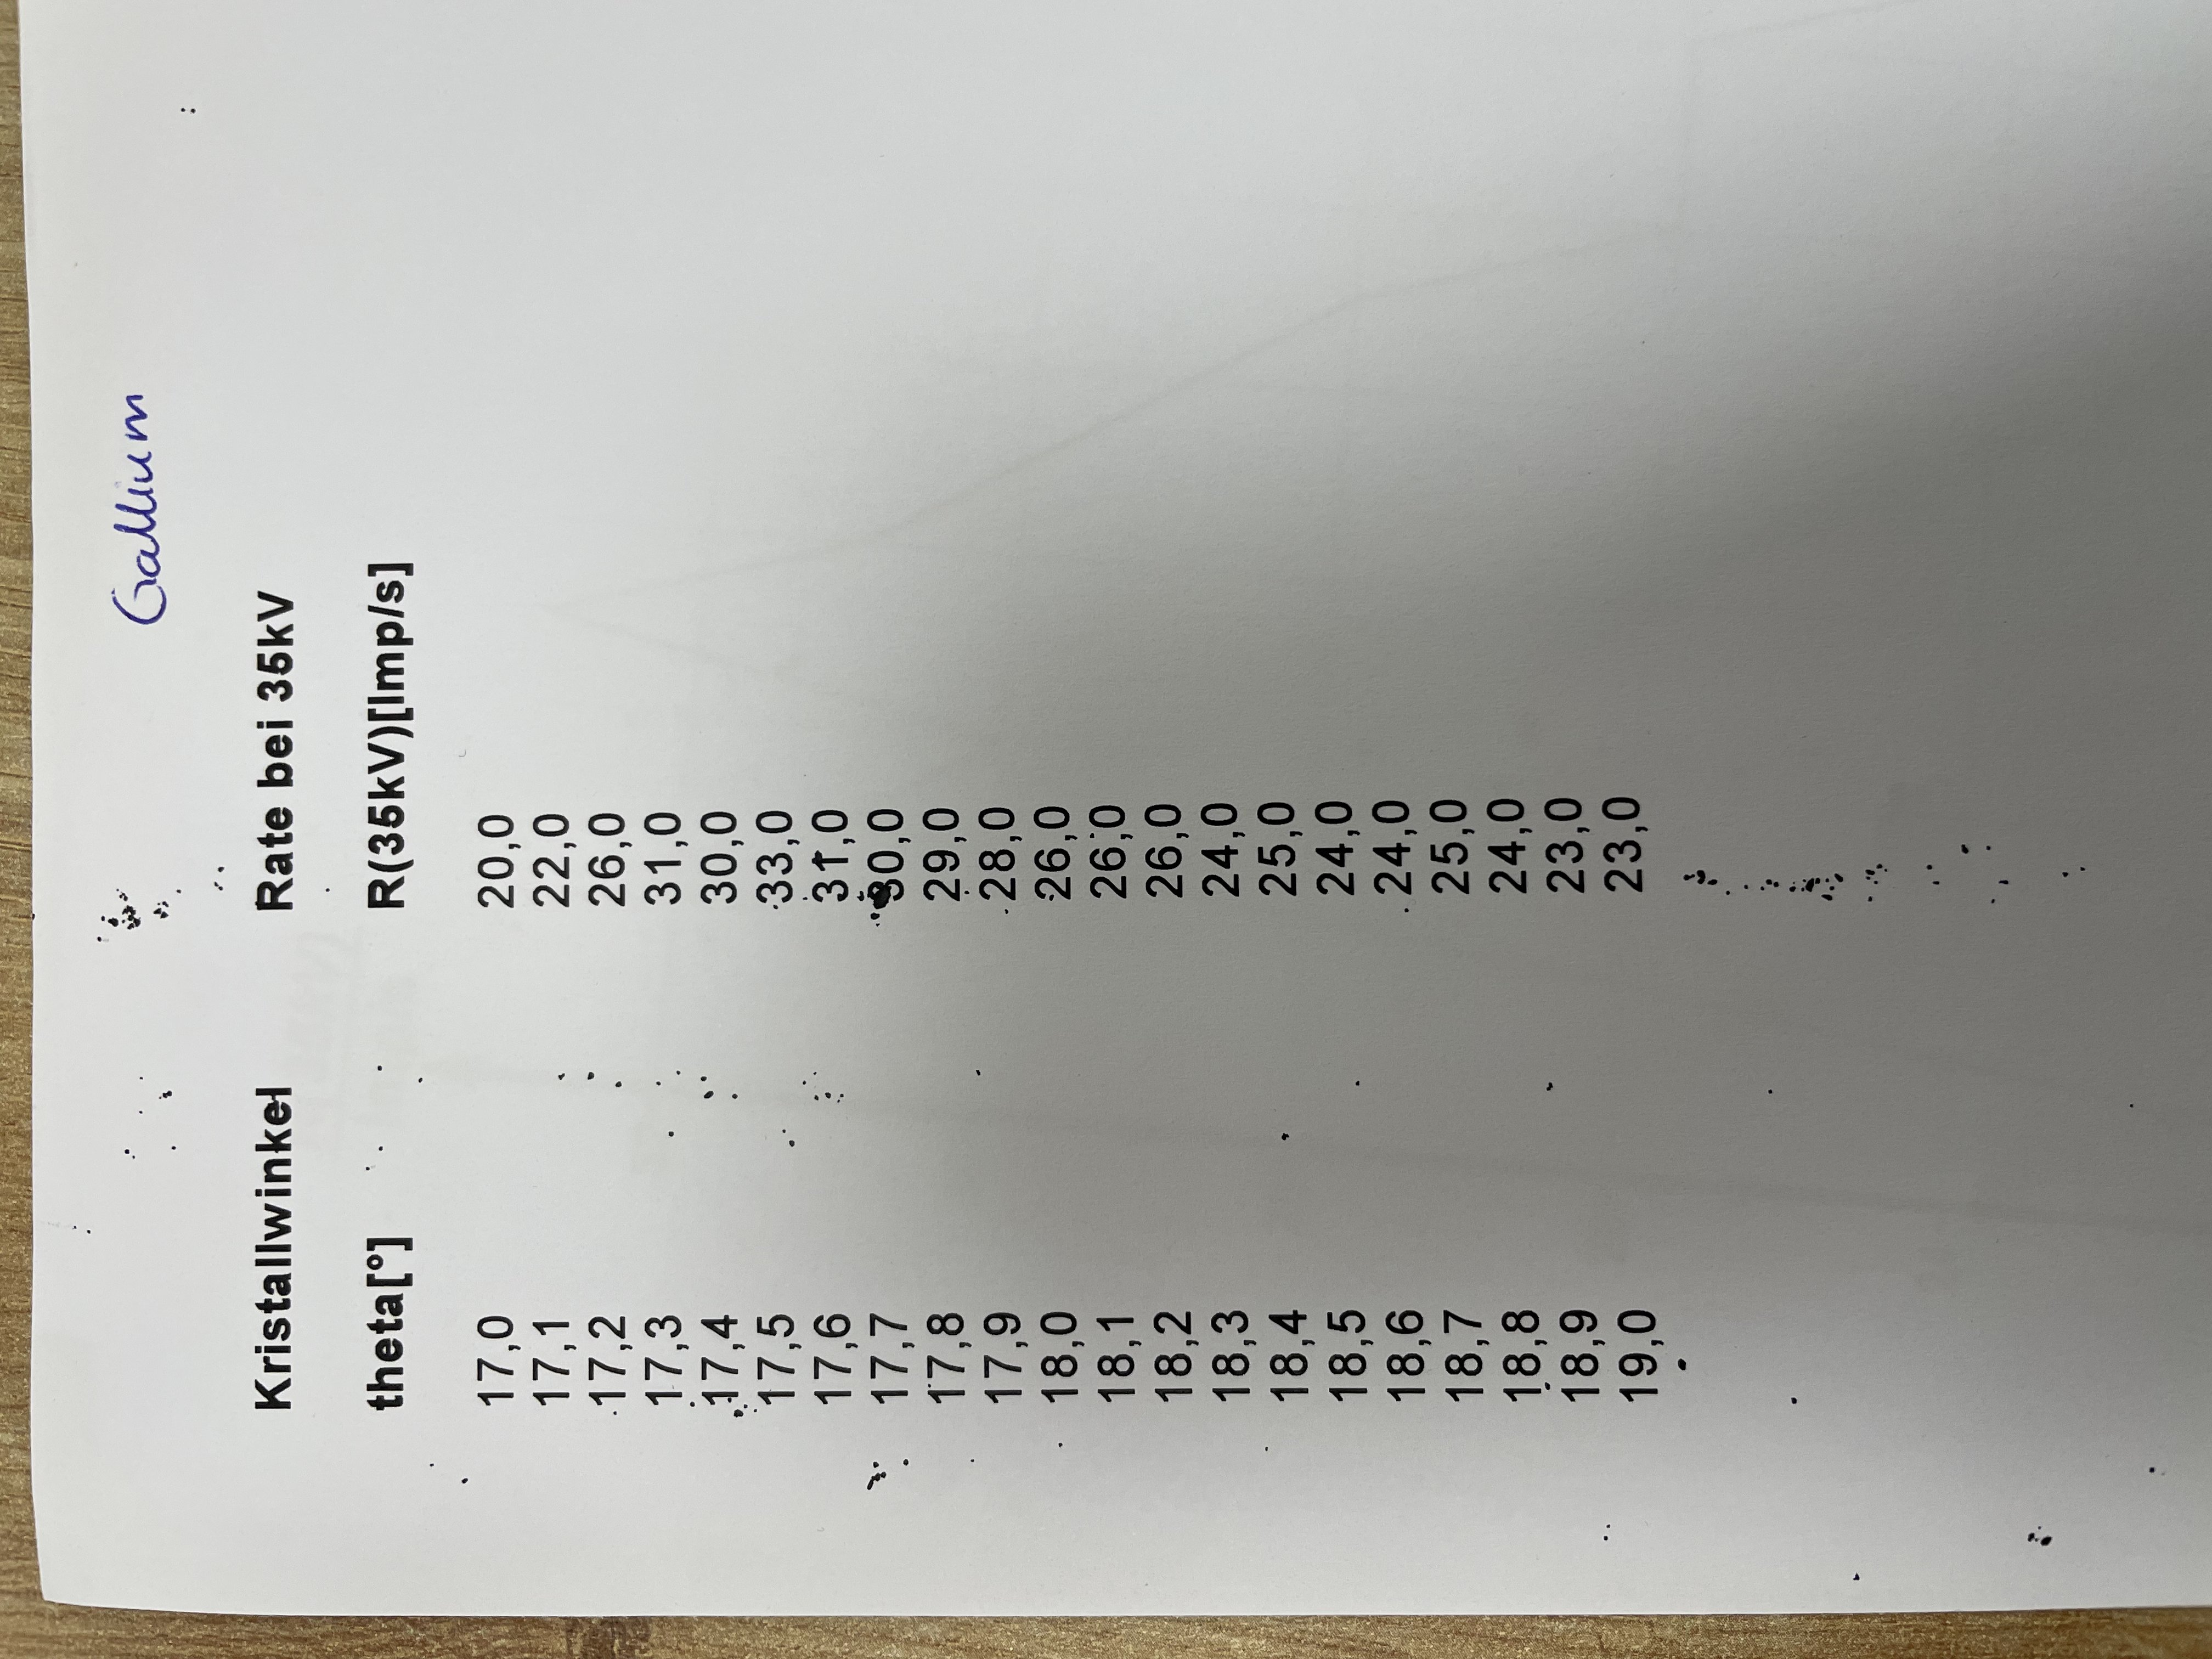
\includegraphics[width=\textwidth, angle=270, origin=c]{"content/Bilder/Gallium.jpg"}
    \caption{Messdaten für den Gallium-Absorber.}
    \label{fig:Messungen_5}
  \end{figure}
  \begin{figure}[H]
    \centering
    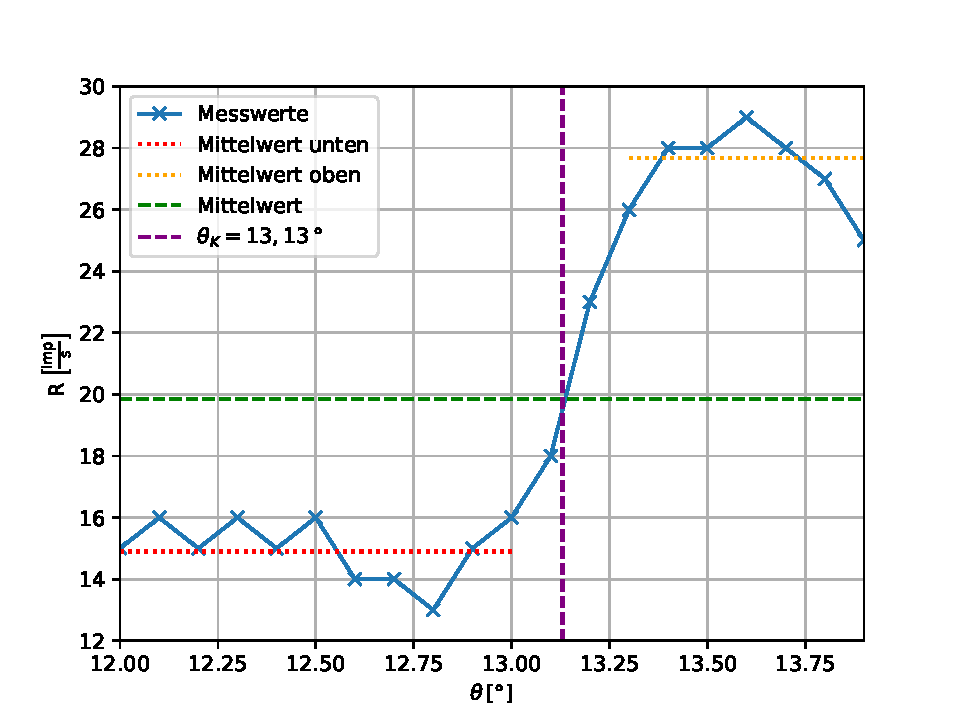
\includegraphics[width=\textwidth, angle=270, origin=c]{"content/Bilder/Brom.jpg"}
    \caption{Messdaten für den Brom-Absorber.}
    \label{fig:Messungen_6}
  \end{figure}
  \begin{figure}[H]
    \centering
    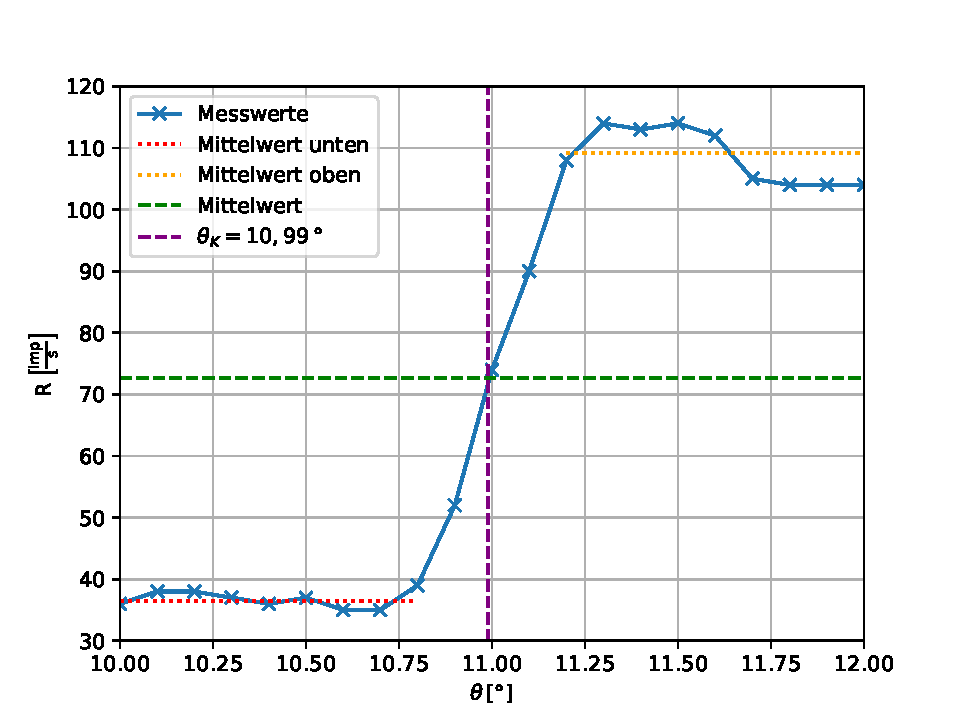
\includegraphics[width=\textwidth, angle=270, origin=c]{"content/Bilder/Strontium.jpg"}
    \caption{Messdaten für den Strontium-Absorber.}
    \label{fig:Messungen_7}
  \end{figure}
  \begin{figure}[H]
    \centering
    \includegraphics[width=\textwidth, angle=270, origin=c]{"content/Bilder/Zirconium.jpg"}
    \caption{Messdaten für den Zirconium-Absorber.}
    \label{fig:Messungen_8}
  \end{figure}
% \begin{figure}[H]
%   \centering
%   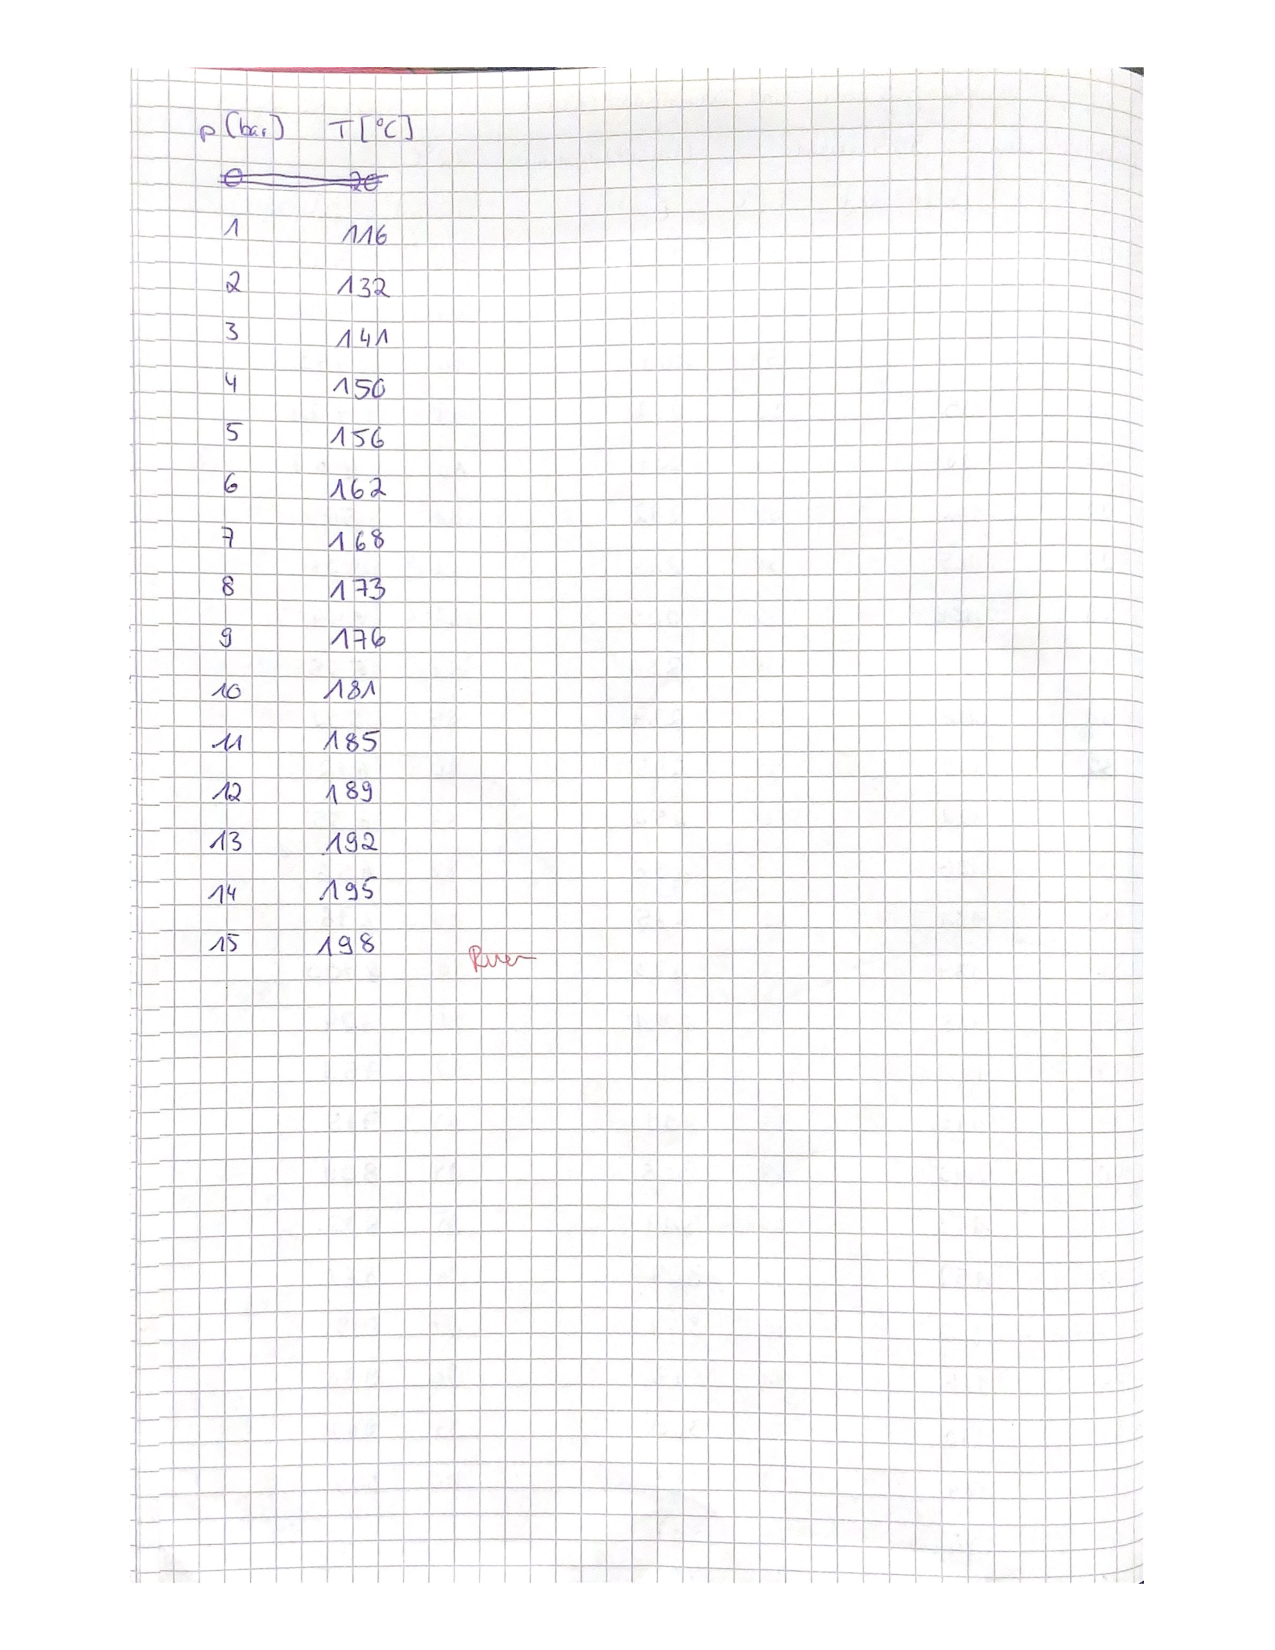
\includegraphics[width=\textwidth]{Messwerte_2.pdf}
%   \label{fig:Messungen_2}
% \end{figure}
% \end{figure}
% \begin{figure}[H]
%   \centering
%   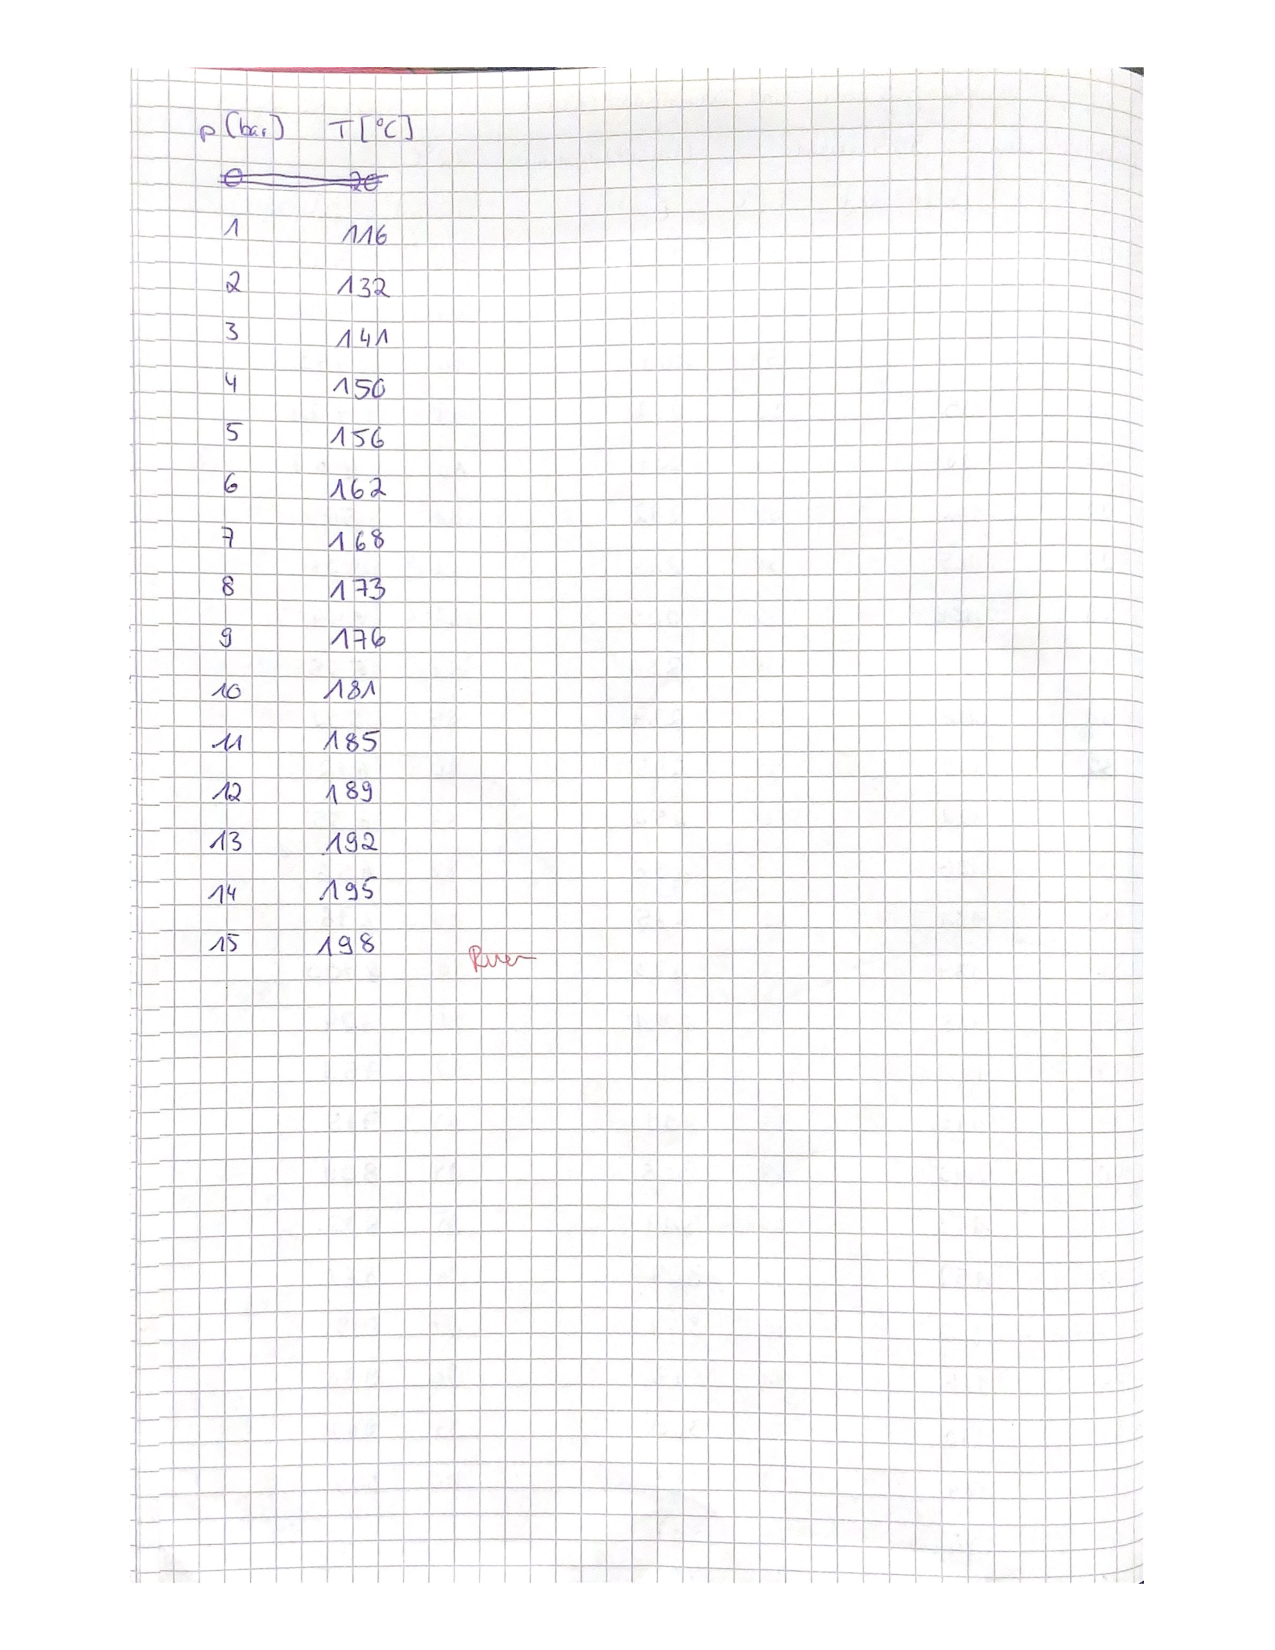
\includegraphics[width=\textwidth]{Messwerte_2.pdf}
%   \label{fig:Messungen_3}
% \end{figure}